\chapter{Documentation Technique}
    (\emph{Description de l'analyse du fichier source})    

    \section{Base de donnée}
        \subsection{Nettoyage du ficher source}
            Le fichier ressource qui nous avaient était fournis (\ilc{credit\_card\_fraud.csv}) avait eu besoin d'un petit nettoyage :
            \begin{bullet-enum}
                \item Les guillemets on étaient supprimées;
                \item Les virgules ont étaient replacés par des point, pour que les nombres soient proprement interprétés par la \ilc{DataFrame};
                \item Les points-virgules furent replacés simplement par des virgules;
                \item Les attributs de types numérique, ont étaient convertis en \ilc{float} ou en \ilc{int};
                \item Les valeurs des champs \ilc{nameOrig} et \ilc{nameDest}, furent convertis en numérique avec le script :
                \begin{pybox}
                    def replace_first_letter(value):
                        if value.startswith('C'):
                            return '1' + value[1:]
                        elif value.startswith('M'):
                            return '2' + value[1:]
                        else:
                            return value
                \end{pybox}
            \end{bullet-enum}

        \subsection{MCD}
            La construction de la base de données a commencé par la réalisation du MCD, et par le passage au MPD avec le logiciel \textbf{Looping}.
            Une fois celui-ci terminé, nous avons utilisé le module \ilc{mysql.connector} pour établir une connexion, et pour la construction de notre base de données depuis Python.
            \begin{figure}[h]
                \centering
                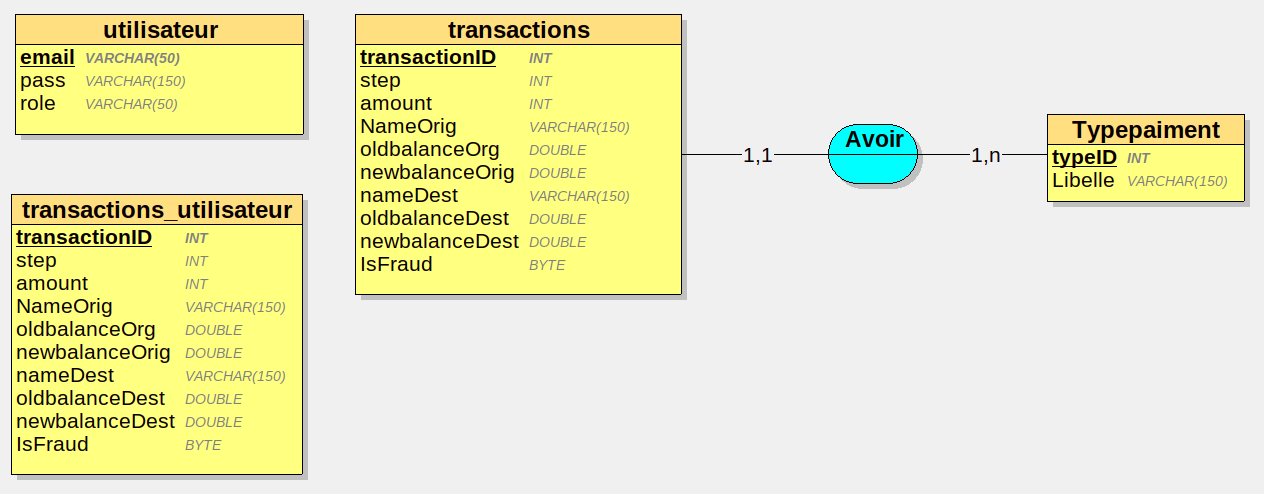
\includegraphics[width=0.8\linewidth]{\pres/db_mcd.png}
                \caption{MCD à partir du fichier \ilc{credit\_card\_fraud.csv}}
            \end{figure}

        \subsection{MLD}
            \begin{sqlbox}
                typepaiment = (
                    typeID INT,
                    libelle VARCHAR(150)
                );

                utilisateur = (
                    email VARCHAR(50),
                    pass VARCHAR(150),
                    role VARCHAR(50)
                );

                transactions_utilisateur = (
                    transactionID INT,
                    step INT,
                    amount INT,
                    nameOrig VARCHAR(150),
                    oldbalanceOrg DOUBLE,
                    newbalanceOrig DOUBLE,
                    nameDest VARCHAR(150),
                    oldbalanceDest DOUBLE,
                    newbalanceDest DOUBLE,
                    isFraud BYTE
                );
                    
                transactions = (
                    transactionID INT,
                    step INT,
                    amount INT,
                    nameOrig VARCHAR(150),
                    oldbalanceOrg DOUBLE,
                    newbalanceOrig DOUBLE,
                    nameDest VARCHAR(150),
                    oldbalanceDest DOUBLE,
                    newbalanceDest DOUBLE,
                    isFraud BYTE, 
                    #typeID
                );
            \end{sqlbox}

    \section{Construction des modèles}
        Après avoir étudié soigneusement les données fournies, nous avons considéré quatre modèles qui pouvaient convenir au dataset: \ilc{XGBoost}, \ilc{AdaBoost}, \ilc{KNN} ainsi que \ilc{RandomForest}.

        \subsection{Entrainement des modèles}
            L'entrainement de chaque modèles \ilc{XGBoost}, \ilc{KNN} et \ilc{RandomForest} a était fait par la méthode \ilc{GridSearchCV}, tandis que le modèle \ilc{AdaBoost} fut simplement entrainer avec \ilc{StratifiedKFold}. Voici la liste des hyperparamètres choisis pour chacun des modèles :
            
            \begin{bluebox}[XGBoost]
                \begin{diamond-enum}
                    \item $1000 \leqslant$ \ilc{n\_estimators} $\leqslant 1400$
                    \item $7 \leqslant$ \ilc{max\_depth} $\leqslant 9$
                \end{diamond-enum}
                \nextenv
                \emph{Le meilleur des estimateur pour ce dataset a été :} 
            \end{bluebox}

            \begin{bluebox}[KNN]
                \begin{diamond-enum}
                    \item $2 \leqslant$ \ilc{n\_neighbors} $\leqslant 11$
                    \item \ilc{weights} $\in$ \ilc{[\textquotesingle uniform\textquotesingle, \textquotesingle distance\textquotesingle]}
                    \item \ilc{p} $\in$ \ilc{[1, 2]}
                    \item \ilc{algorith} $\in$ \ilc{[\textquotesingle ball\_tree\textquotesingle, \textquotesingle kd\_tree\textquotesingle]}
                \end{diamond-enum}
                \nextenv
                \emph{Le meilleur des estimateur pour ce dataset a été :}
            \end{bluebox}

            \begin{bluebox}[RandomForest]
                \begin{diamond-enum}
                    \item $100 \leqslant$ \ilc{n\_estimators} $\leqslant 300$
                    \item $1 \leqslant$ \ilc{max\_depth} $\leqslant 30$
                    \item \ilc{criterion} $\in$ \ilc{[\textquotesingle entropy\textquotesingle, \textquotesingle gini\textquotesingle]}
                \end{diamond-enum}
                \nextenv
                \emph{Le meilleur des estimateur pour ce dataset a été :} \ilc{n\_estimators} $= 200$, \ilc{criterion} $=$ \ilc{\textquotesingle entropy\textquotesingle}, \ilc{max\_depth} $= 20$.
            \end{bluebox}

        \subsection{Evaluation des modèles}

            \begin{table}[h]
                \begin{tabularx}{\textwidth}{X|XXXXX}
                    \textbf{Modèle}    & \textbf{Accuracy} & \textbf{Precision} & \textbf{Recall} & \textbf{F1 Score} & \textbf{AUC} \\ \hline
                    \ilc{KNN}          &                   &                    &                 &                   &              \\
                    \ilc{XGBoost}      &                   &                    &                 &                   &              \\
                    \ilc{AdaBoost}     &                   &                    &                 &                   &              \\
                    \ilc{RandomForest} &                   &                    &                 &                   &              \\
                \end{tabularx}
                \caption{Métriques calculés pour les modèles entraînés}
            \end{table}

            \begin{figure}[h]
                \centering
                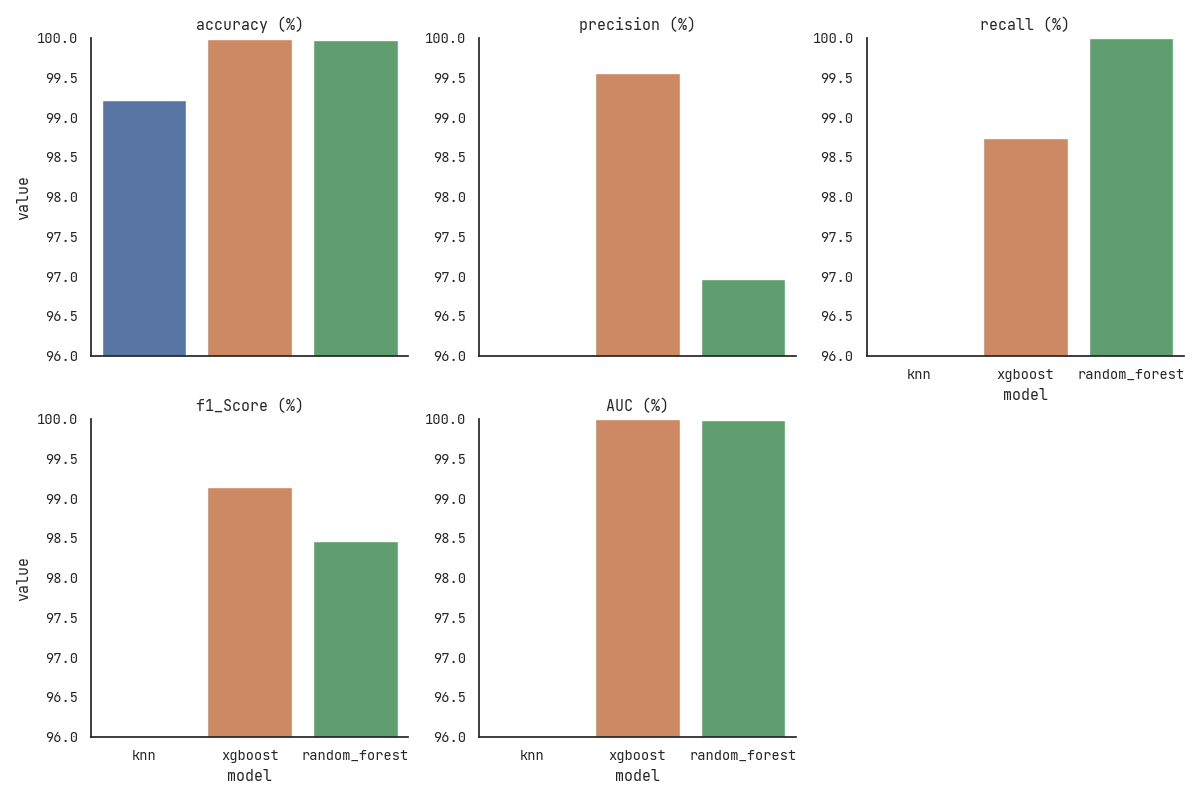
\includegraphics[width=\linewidth]{\pres/all_metrics_plot.png}
                \caption{Comparaison des modèles}
            \end{figure}

        \section{Realisation de l'application}
            La création de l'application a commencé bien évidemment par la création de la maquette, nous avons utilisé le logiciel \textbf{Figma} pour cette tâche.
            Une fois celle-ci réalisée, nous avons commencé par structurer notre projet.

            